\documentclass[border=8pt, multi, tikz]{standalone}
%\usepackage{blocks}
\usepackage{import}
\usetikzlibrary{3d}
\subimport{layers/}{init}
\usetikzlibrary{positioning}

\def\ConvColor{rgb:yellow,5;red,2.5;white,5}
\def\ConvReluColor{rgb:yellow,5;red,5;white,5}
\def\PoolColor{rgb:red,1;black,0.3}
\def\UnpoolColor{rgb:blue,2;green,1;black,0.3}
\def\FcColor{rgb:blue,5;red,2.5;white,5}
\def\FcReluColor{rgb:blue,5;red,5;white,4}
\def\SoftmaxColor{rgb:magenta,5;black,7}


\newcommand{\copymidarrow}{\tikz \draw[-Stealth,line width =0.8mm,draw={rgb:blue,4;red,1;green,1;black,3}] (-0.3,0) -- ++(0.3,0);}

\begin{document}
\begin{tikzpicture}
\tikzstyle{connection}=[ultra thick,every node/.style={sloped,allow upside down},draw=\edgecolor,opacity=0.7]
\tikzstyle{copyconnection}=[ultra thick,every node/.style={sloped,allow upside down},draw={rgb:blue,4;red,1;green,1;black,3},opacity=0.7]

%%%%%%%%%%%%%%%%%%%%%%%%%%%%%%%%%%%%%%%%%%%%%%%%%%%%%%%%%%%%%%%%%%%%%%%%%%%%%%%%%%%%%%%%
%% Draw Encoder
%%%%%%%%%%%%%%%%%%%%%%%%%%%%%%%%%%%%%%%%%%%%%%%%%%%%%%%%%%%%%%%%%%%%%%%%%%%%%%%%%%%%%%%%
% conv1_1,conv1_2
\pic[shift={(0,0,0)}] at (0,0,0) {RightBandedBox={name=cr1,%
        xlabel={{"1","3"}},zlabel=128,fill=\ConvColor,bandfill=\ConvReluColor,%
        height=40,width={2,2},depth=40}};
%conv->batch->relu>convtransp->batch->relu
\pic[shift={(3,0,0)}] at (0,0,0) {RightBandedBox={name=cr1,%
        xlabel={{"64","64"}},zlabel=128,fill=\ConvColor,bandfill=\ConvReluColor,%
        height=40,width={2,2},depth=40}};
%pool1
\pic[shift={(0,0,0)}] at (cr1-east) {Box={name=p1,%
        fill=\PoolColor,opacity=0.5,height=32,width=1,depth=32}};
%%%%%%%%%%
% conv2_1,conv2_2
\pic[shift={(2.5,0,0)}] at (p1-east) {RightBandedBox={name=cr2,%
        xlabel={{"128","128"}},zlabel=64,fill=\ConvColor,bandfill=\ConvReluColor,%
        height=32,width={3.5,3.5},depth=32}};
%pool2
\pic[shift={(0,0,0)}] at (cr2-east) {Box={name=p2,%
        fill=\PoolColor,opacity=0.5,height=25,width=1,depth=25}};
%%%%%%%%%%
% conv3_1,conv3_2
\pic[shift={(2.0,0,0)}] at (p2-east) {RightBandedBox={name=cr3,%
        xlabel={{"256","256"}},zlabel=32,fill=\ConvColor,bandfill=\ConvReluColor,%
        height=25,width={4.5,4.5},depth=25}};
%pool3
\pic[shift={(0,0,0)}] at (cr3-east) {Box={name=p3,%
        fill=\PoolColor,opacity=0.5,height=16,width=1,depth=16}};
%%%%%%%%%%
% conv4_1,conv4_2,conv4_3
\pic[shift={(1.5,0,0)}] at (p3-east) {RightBandedBox={name=cr4,%
        xlabel={{"512","512"}},zlabel=16,fill=\ConvColor,bandfill=\ConvReluColor,%
        height=16,width={6,6},depth=16}};
%pool4
\pic[shift={(0,0,0)}] at (cr4-east) {Box={name=p4,%
        fill=\PoolColor,opacity=0.5,height=8,width=1,depth=8}};
%%%%%%%%%%%%%%%%%%%%%%%%%%%%%%%%%%%%%%%%%%%%%%%%%%%%%%%%%%%%%%%%%%%%%%%%%%%%%%%%%%%%%%%%
%% Bottleneck
%%%%%%%%%%%%%%%%%%%%%%%%%%%%%%%%%%%%%%%%%%%%%%%%%%%%%%%%%%%%%%%%%%%%%%%%%%%%%%%%%%%%%%%%% conv5_1,conv5_2,conv5_3
\pic[shift={(1.00,0,0)}] at (p4-east) {RightBandedBox={name=cr5,%
        xlabel={{"512","512"}},zlabel=8,fill=\ConvColor,bandfill=\ConvReluColor,%
        height=8,width={6,6},depth=8}};
%%%%%%%%%%%%%%%%%%%%%%%%%%%%%%%%%%%%%%%%%%%%%%%%%%%%%%%%%%%%%%%%%%%%%%%%%%%%%%%%%%%%%%%%
%% Draw Decoder 
%%%%%%%%%%%%%%%%%%%%%%%%%%%%%%%%%%%%%%%%%%%%%%%%%%%%%%%%%%%%%%%%%%%%%%%%%%%%%%%%%%%%%%%%
%% unpool4, 
\pic[shift={(1.2,0,0)}] at (cr5-east) {RightBandedBox={name=up4,
        xlabel={{"512", "dummy"}},fill=\ConvColor,opacity=0.6,height=16,width=6,depth=16, bandfill=\ConvReluColor}};
\pic[shift={(0,0,0)}] at (up4-east) {RightBandedBox={name=ucr4a,%
        xlabel={{"512","dummy"}},fill=\ConvColor,bandfill=\ConvReluColor,
        height=16,width=6,depth=16}};
\pic[shift={(0.0,0,0)}] at (ucr4a-east) {Box={name=up2,%
        fill=\UnpoolColor,opacity=0.6,height=16,width=1,depth=16,zlabel=16}};
%\pic[shift={(0,0,0)}] at (ucr4-east) {RightBandedBox={name=cat4,%
%        xlabel={{"512",""}},fill={rgb:white,1;black,3},bandfill={rgb:white,1;black,2},opacity=0.2,height=16,width=6,depth=16}};    
%\pic[shift={(0,0,0)}] at (cat4-east) {RightBandedBox={name=ucr4a,%
%        xlabel={{"512","512"}},zlabel=16,fill=\ConvColor,bandfill=\ConvReluColor,%
%        height=16,width={6,6},depth=16}};
%%%%%%%%%%
%% unpool3, 
\pic[shift={(1.8,0,0)}] at (ucr4a-east) {RightBandedBox={name=up3,%
        xlabel={{"256", "dummy"}},fill=\ConvColor,opacity=0.6,height=25,width=4.5,depth=25, bandfill=\ConvReluColor}};
\pic[shift={(0,0,0)}] at (up3-east) {RightBandedBox={name=ucr3a,%
        xlabel={{"256","dummy"}},fill=\ConvColor,bandfill=\ConvReluColor,%
        height=25,width=4.5,depth=25}};
\pic[shift={(0.0,0,0)}] at (ucr3a-east) {Box={name=up2,%
        fill=\UnpoolColor,opacity=0.6,height=25,width=1,depth=25,zlabel=32}};
%\pic[shift={(0,0,0)}] at (ucr3-east) {RightBandedBox={name=cat3,%
%        xlabel={{"256",""}},fill={rgb:white,1;black,3},bandfill={rgb:white,1;black,2},opacity=0.2,height=25,width=4.5,depth=25}};
%\pic[shift={(0,0,0)}] at (cat3-east) {RightBandedBox={name=ucr3a,%
%        xlabel={{"256","256"}},zlabel=32,fill=\ConvColor,bandfill=\ConvReluColor,%
%        height=25,width={4.5,4.5},depth=25}};
%%%%%%%%%%
%% unpool2, 
\pic[shift={(2.2,0,0)}] at (ucr3a-east) {RightBandedBox={name=up2,%
        xlabel={{"128","dummy"}},fill=\ConvColor,bandfill=\ConvReluColor,opacity=0.6,height=32,width=3.5,depth=32}};
\pic[shift={(0,0,0)}] at (up2-east) {RightBandedBox={name=ucr2a,%
        xlabel={{"128","dummy"}},fill=\ConvColor,bandfill=\ConvReluColor,%
        height=32,width=3.5,depth=32}};
\pic[shift={(0.0,0,0)}] at (ucr2a-east) {Box={name=up1,%
        fill=\UnpoolColor,opacity=0.6,height=32,width=1,depth=32,zlabel=64}};
%\pic[shift={(0,0,0)}] at (ucr2-east) {RightBandedBox={name=cat2,%
%        xlabel={{"128",""}},fill={rgb:white,1;black,3},bandfill={rgb:white,1;black,2},opacity=0.2,height=32,width=3.5,depth=32}};    
%\pic[shift={(0,0,0)}] at (cat2-east) {RightBandedBox={name=ucr2a,%
%        xlabel={{"128","128"}},zlabel=64,fill=\ConvColor,bandfill=\ConvReluColor,%
%        height=32,width={3.5,3.5},depth=32}};
%%%%%%%%%%
%% unpool1, 
\pic[shift={(2.5,0,0)}] at (ucr2a-east) {RightBandedBox={name=up1,%
        xlabel={{"64","dummy"}},fill=\ConvColor,bandfill=\ConvReluColor,opacity=0.6,height=32,width=2.5,depth=32}};
\pic[shift={(0,0,0)}] at (up1-east) {RightBandedBox={name=ucr1a,%
        xlabel={{"64","dummy"}},fill=\ConvColor,bandfill=\ConvReluColor,%
        height=32,width=2.5,depth=32}};
\pic[shift={(0.0,0,0)}] at (ucr1a-east) {Box={name=up0,%
        fill=\UnpoolColor,opacity=0.6,height=32,width=1,depth=32,zlabel=64}};
%\pic[shift={(0,0,0)}] at (ucr1-east) {RightBandedBox={name=cat1,%
%        xlabel={{"64",""}},fill={rgb:white,1;black,3},bandfill={rgb:white,1;black,2},opacity=0.2,height=40,width=2.5,depth=40}};  
%\pic[shift={(0,0,0)}] at (cat1-east) {RightBandedBox={name=ucr1a,%
%        xlabel={{"64","64"}},fill=\ConvColor,bandfill=\ConvReluColor,%
%        height=40,width={2.5,2.5},depth=40}};
%%%%%%%%%%%%%%%%%%%%%%%%%%%%%%%%%%%%%%%%%%%%%%%%%%%%%%%%%%%%%%%%%%%%%%%%%%%%%%%%%%%%%%%%
%% Self-attention and end
%%%%%%%%%%%%%%%%%%%%%%%%%%%%%%%%%%%%%%%%%%%%%%%%%%%%%%%%%%%%%%%%%%%%%%%%%%%%%%%%%%%%%%%%%
\pic[shift={(1.75,0,0)}] at (ucr1a-east) {Box={name=out,%
        xlabel={{"64", "dummy"}},fill=\SoftmaxColor,height=32,width=2.5,depth=32}};
\pic[shift={(0,0,0)}] at (out-east) {RightBandedBox={name=out1,%
        xlabel={{"64", "dummy"}},bandfill=\ConvReluColor,fill=\ConvColor,height=32,width=2.5,depth=32,zlabel=64}};
\pic[shift={(2.5,0,0)}] at (out-east) {Box={name=out2,%
        xlabel={{"3", "dummy"}},fill=\ConvColor,height=40,width=1,depth=40,zlabel=128}};
%%%%%%%%%%%%%%%%%%%%%%%%%%%%%%%%%%%%%%%%%%%%%%%%%%%%%%%%%%%%%%%%%%%%%%%%%%%%%%%%%%%%%%%
% Draw connections
%%%%%%%%%%%%%%%%%%%%%%%%%%%%%%%%%%%%%%%%%%%%%%%%%%%%%%%%%%%%%%%%%%%%%%%%%%%%%%%%%%%%%%%

\node[canvas is zy plane at x=0] (temp) at (40,0,0) {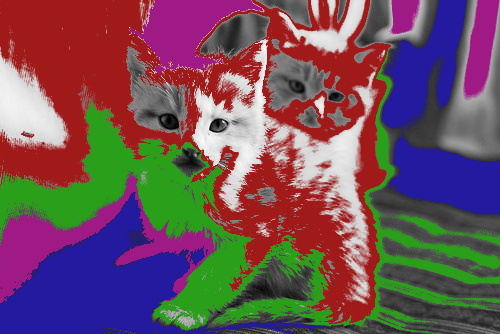
\includegraphics[width=8cm,height=8cm]{cats_col.jpg}};

\draw [connection]  (p1-east)    -- node {\midarrow} (cr2-west);
\draw [connection]  (p2-east)    -- node {\midarrow} (cr3-west);
\draw [connection]  (p3-east)    -- node {\midarrow} (cr4-west);
\draw [connection]  (p4-east)    -- node {\midarrow} (cr5-west);
\draw [connection]  (cr5-east)   -- node {\midarrow} (up4-west);
\draw [connection]  (ucr4a-east) -- node {\midarrow} (up3-west);
\draw [connection]  (ucr3a-east) -- node {\midarrow} (up2-west);
\draw [connection]  (ucr2a-east) -- node {\midarrow} (up1-west);
\draw [connection]  (ucr1a-east) -- node {\midarrow} (out-west);
\draw [connection]  (out1-east) -- node {\midarrow} (out2-west);
%\draw [connection]  (out-east)   -- node {\midarrow} ++(2,0,0);

\path (cr4-southeast) -- (cr4-northeast) coordinate[pos=1.25] (cr4-top) ;
\path (cr3-southeast) -- (cr3-northeast) coordinate[pos=1.25] (cr3-top) ;
\path (cr2-southeast) -- (cr2-northeast) coordinate[pos=1.25] (cr2-top) ;
\path (cr1-southeast) -- (cr1-northeast) coordinate[pos=1.25] (cr1-top) ;

\path (ucr4a-south)  -- (ucr4a-north)  coordinate[pos=1.67] (cat4-top) ;
%\path (cat4-south)  -- (cat4-north)  coordinate[pos=1.67] (cat4-top) ;
\path (up4-south)  -- (up4-north)  coordinate[pos=1.67] (cat4-top) ;
%\path (cat4-south)  -- (cat4-north)  coordinate[pos=1.67] (cat4-top) ;
\path (up3-south)  -- (up3-north)  coordinate[pos=1.46] (cat3-top) ;
%\path (cat3-south)  -- (cat3-north)  coordinate[pos=1.46] (cat3-top) ;
\path (up2-south)  -- (up2-north)  coordinate[pos=1.44] (cat2-top)  ;
%\path (cat2-south)  -- (cat2-north)  coordinate[pos=1.44] (cat2-top)  ;
\path (ucr1a-south)  -- (ucr1a-north)  coordinate[pos=1.25] (cat1-top)  ;
%\path (cat1-south)  -- (cat1-north)  coordinate[pos=1.25] (cat1-top)  ;
%
%\draw [copyconnection]  (cr4-northeast)  
%-- node {\copymidarrow}(cr4-top)
%-- node {\copymidarrow}(cat4-top)
%-- node {\copymidarrow} (cat4-north);
%
\draw [copyconnection]  (cr3-northeast)  
-- node {\copymidarrow}(cr3-top)
-- node {\copymidarrow}(cat4-top)
-- node {\copymidarrow} (up4-north);
%-- node {\copymidarrow} (cat4-north);
%
\draw [copyconnection]  (cr2-northeast)  
-- node {\copymidarrow}(cr2-top)
-- node {\copymidarrow}(cat3-top)
-- node {\copymidarrow} (up3-north);
%-- node {\copymidarrow} (cat3-north);
%
\draw [copyconnection]  (cr1-northeast)  
-- node {\copymidarrow}(cr1-top)
-- node {\copymidarrow}(cat2-top)
-- node {\copymidarrow} (up2-north);
%-- node {\copymidarrow} (cat2-north);

%%%%%%%%%%%%%%%%%%%%%%%%%%%%%%%%%%%%%%%%%%%%%%%%%%%%%%%%%%%%%%%%%%%%%%%%%%%%%%%%%%%%%%%
% discriminator
\pic[shift={(3,0,0)}] at (7,-13,0) {Box={name=dis0,%
        xlabel={{"3","dummy"}},zlabel=128,fill=\ConvColor,
        height=40,width={1},depth=40}};
\pic[shift={(2.5,0,0)}] at (dis0-east) {RightBandedBox={name=dis1,%
        xlabel={{"64","64"}},zlabel=64,fill=\ConvColor,bandfill=\ConvReluColor,%
        height=32,width={2},depth=32}};

\pic[shift={(2.0,0,0)}] at (dis1-east) {RightBandedBox={name=dis2,%
        xlabel={{"128","128"}},zlabel=32,fill=\ConvColor,bandfill=\ConvReluColor,%
        height=25,width={3.5},depth=25}};

\pic[shift={(1.5,0,0)}] at (dis2-east) {RightBandedBox={name=dis3,%
        xlabel={{"256","256"}},zlabel=16,fill=\ConvColor,bandfill=\ConvReluColor,%
        height=16,width={4.5},depth=16}};

\pic[shift={(1.3,0,0)}] at (dis3-east) {RightBandedBox={name=dis4,%
        xlabel={{"256","256"}},zlabel=8,fill=\ConvColor,bandfill=\ConvReluColor,%
        height=8,width={4.5},depth=8}};

\pic[shift={(1.3,0,0)}] at (dis4-east) {RightBandedBox={name=dis5,%
        xlabel={{"512","256"}},zlabel=4,fill=\ConvColor,bandfill=\ConvReluColor,%
        height=8,width={8},depth=8}};

\pic[shift={(1.3,0,0)}] at (dis5-east) {Box={name=dis6,%
        xlabel={{"512","256"}},zlabel=4,fill=\SoftmaxColor,
        height=8,width={8},depth=8}};

\pic[shift={(1.3,0,0)}] at (dis6-east) {Box={name=dis7,%
        xlabel={{"512","256"}},zlabel=4,fill=\ConvColor,
        height=8,width={8},depth=8}};

\pic[shift={(1.3,0,0)}] at (dis7-east) {Box={name=dis8,%
        xlabel={{"512","256"}},zlabel=1,fill=\ConvColor,
        height=4,width={8},depth=4}};

\pic[shift={(1.3,0,0)}] at (dis8-east) {Box={name=dis9,%
        xlabel={{"1","256"}},fill=\ConvColor,
        height=1,width={1},depth=1}};

%%%%%%%%%%%%%%%%%%%%%%%%%%%%%%%%%%%%%%%%%%%%%%%%%%%%%%%%%%%%%%%%%%%%%%%%%%%%%%%%%%%%%%%
% connections
\draw [connection]  (dis0-east)    -- node {\midarrow} (dis1-west);
\draw [connection]  (dis1-east)    -- node {\midarrow} (dis2-west);
\draw [connection]  (dis2-east)    -- node {\midarrow} (dis3-west);
\draw [connection]  (dis3-east)    -- node {\midarrow} (dis4-west);
\draw [connection]  (dis4-east)    -- node {\midarrow} (dis5-west);
\draw [connection]  (dis5-east)    -- node {\midarrow} (dis6-west);
\draw [connection]  (dis6-east)    -- node {\midarrow} (dis7-west);
\draw [connection]  (dis7-east)    -- node {\midarrow} (dis8-west);

%%%%%%%%%%%%%%%%%%%%%%%%%%%%%%%%%%%%%%%%%%%%%%%%%%%%%%%%%%%%%%%%%%%%%%%%%%%%%%%%%%%%%%%
% between, before, after networks
%\draw [connection]  (out2-east) -- node {\midarrow} (dis0-west);

\path (out2-north) -- (out2-south) coordinate[pos=1.28] (bot-gen) ;
\path (dis0-south) -- (dis0-north) coordinate[pos=1.35] (top-dis) ;
\path (bot-gen) -- (top-dis) coordinate[pos=1.174] (custom-dis) ;
\path (dis0-east) -- (dis0-west) coordinate[pos=25.45] (east-dis) ;

\draw [copyconnection]  (out2-east)  
-- node {\copymidarrow}(40,0,0)
-- node {\copymidarrow}(40,-5,0)
-- node {\copymidarrow}(40,-6.2,0)
-- node {\copymidarrow}(top-dis)
-- node {\copymidarrow}(custom-dis)
-- node {\copymidarrow}(east-dis)
-- node {\copymidarrow} (dis0-west);

\node[canvas is zy plane at x=0] (temp) at (-3,-13,0) {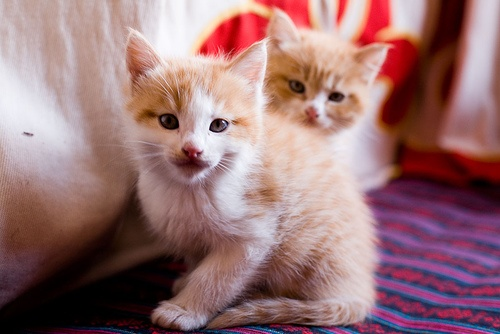
\includegraphics[width=8cm,height=8cm]{cats.jpg}};
\node[canvas is zy plane at x=0] (temp) at (-5,0,0) {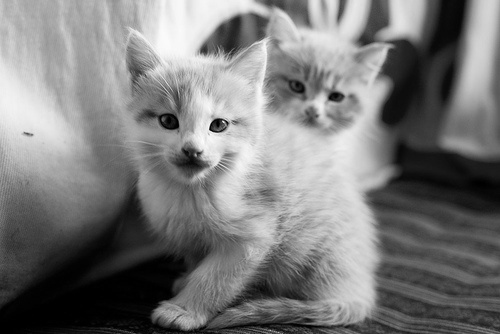
\includegraphics[width=8cm,height=8cm]{cats_bw.jpg}};
%\node[canvas is zy plane at x=0] (temp) at (40,0,0) {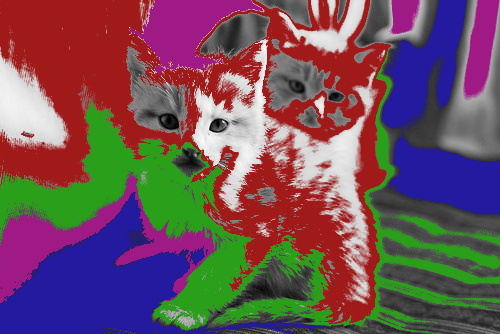
\includegraphics[width=8cm,height=8cm]{cats_col.jpg}};
\draw [connection]  (-1,-13,0)    -- node {\midarrow} (dis0-west);
\draw [connection]  (-4,0,0)    -- node {\midarrow} (-1.5,0,0);
\draw [connection]  (0.5,0,0)    -- node {\midarrow} (cr1-west);

%true false
\draw [connection]  (dis8-east)    -- node {\midarrow} (33.0,-13,0);
\draw [connection]  (33.7,-13,0)    -- node {\midarrow} (35,-13,0);
\draw [connection]  (35,-13,0)    -- node {\midarrow} (35,-11,0);
\draw [connection]  (35,-13,0)    -- node {\midarrow} (35,-15,0);

\node at (35,-10,0) {\Huge Fake};
\node at (35,-16,0) {\Huge Real};


\end{tikzpicture}
\end{document}
